\section{Extensions}
\label{sec:extensions}

In section \ref{sec:approach} 
  we made some simplifications in order to keep the discussion brief.
We discuss three extensions to our base approach.
The first extension provides further details on how to assess
  identity conditions of typed literals, which may occur in the object
  position of a triple.
The second extension generalizes the notion of a
  predicate, allowing more indiscernibility predicates to be found.
The third extension shows that definitions
  \ref{def:identity_lower_approximation} and
  \ref{def:identity_higher_approximation}
  do not give the most optimal solution in some arcane cases.

\subsection{Identity of typed literals}

In order to deal with predefined datatypes such as integers, dates, etc.,
  RDF introduces the notion of ``typed literals''.
For such typed literals, identity does not suffice in order to ascertain
  that the sets of object terms denote the same resources
  (definition \ref{def:indiscernibility_properties}).
The reason for this is that typed literals have special identity conditions.
Since typed literals are quite common in SW data, we elaborate on this here.
Roughly speaking, for typed literals we assume a lexical-to-value mapping
  \cite{Hayes2004}, which assigns a value to each lexical expression.
For each datatype we assume a datatype-specific identity relation
  partitioning the datatype's value space.
Identity between typed literals is then defined
  as the datatype-specific identity between the values of the literals
  under the lexical-to-value mapping.
This extension was already used to perform the computational
  experiment of section \ref{sec:experiment}.

\begin{comment}
First we assume a datatype map
  \mbox{$D : \mathcal{I} \rightarrow ICEXT(I({\small \texttt{rdfs:Datatype}}))$},
  where $ICEXT$ is the functional map from classes onto their instances.
Second, for each datatype $d$ we assume a lexical-to-value mapping
  $L2V(d)$,\cite{Hayes2004},
  %: V(d) \rightarrow LEX(d)
  which assigns a value to each lexical expression.
Finally, for each datatype $d$ we assume a datatype-specific identity relation
  $\sim_d$ partitioning the datatype's value space $V(d)$.\footnote{
    Relation $\sim_d$ poses some problems to implement correctly,
      see section \ref{sec:implementation} for details.
    }

Suppose that two objects $o_1$ and $o_2$ are both typed literals,
  with $o_1 = \pair{d_1}{x_1}$ and $o_2 = \pair{d_2}{x_2}$
  for datatype names $d_1$ and $d_2$ and value names $x_1$ and $x_2$.
Identity between $o_1$ and $o_2$ is then defined as in
  \ref{def:identity_typed_literals}.

\begin{definition}[Identity for typed literals]
\label{def:identity_typed_literals}
\begin{align}
  o_1 \approx o_1
\,\iff\,
    D(d_1) = D(d_2)
  & \; \land \; &\nonumber\\
    x_1 \in LEX(d_1)
  & \; \land \; &\nonumber\\
    x_2 \in LEX(d_2)
  & \; \land \; &\nonumber\\
    l2v(D(d_1))(x_1) \sim_d l2v(D(d_2))(x_2)\nonumber
\end{align}
\end{definition}

\noindent Notice that the datatype-specific lexical-to-value mapping
  in definition \ref{def:identity_typed_literals} is relevant for
  the identification of identity,
  since two lexical expressions may map onto the same value
  according to one datatype but onto different values
  according to another.
An example of this are the lexical expressions $0.1$ and $0.10000000009$,
  which map to the same value according to datatype
  {\small \texttt{xsd:float}}
  but to different values according to datatype
  {\small \texttt{xsd:decimal}} \cite{Goldberg1991}.

In definition \ref{def:identity_typed_literals}
  the conjuncts which state that the value names belong to
  the respective lexical spaces may seem superfluous at first.
But for ill-typed literals,
  i.e. those whose value names do not belong to the lexical space of
  the specified datatype,
  the interpretation is not determined and they are only known to denote
  some arbitrary non-literal value \cite{Hayes2004}.\footnote{
    From the practice of working with SW data, the authors can testify
    that ill-typed literals do occur and are actually quite common!}
\end{comment}


\subsection{Generic properties and property maps}

\subsection{Motivation}

We want to generalize the 

When we look at concrete datasets we see that the resources that make up
  an identity pair do not often share a lot of properties.
The pragmatics reflects this, as identity statements are often used
  to link to other resources and import statements
  (i.e. properties asserted of a resources)
  that are not asserted of the former resource.
However, while there is not too much overlap in properties,
  resources are oftentimes connected at a deeper level,
  via a path that spans two or more properties.

The reason for wanting to extend properties 

\subsection{Conceptual}

For instance the property ``is spoken in'' is denoted by
  the predicate term \verb|IIMBTBOX:spoken_in| in the IIMB dataset.
This relates natural languages to the countries in which they are spoken.

We generalize the notion of a property,
  so that is can be denoted by a sequence of predicate terms.
For example the property ``is spoken in a country whose capital is''
  is denoted by
  $\tuple{\texttt{IIMBTBOX:spoken\_in},\texttt{IIMBTBOX:has\_capital}}$,
  relating natural languages to the capitals of the countries in which
  they are spoken.

\subsection{Theoretical}

For each sequence of predicate terms $\tuplerange{p_1}{p_n}$
  we assume a functional mapping
  $f_{\tuplerange{p_1}{p_n}} : S_G \rightarrow \powerset{O_G}$,
  from subject terms into sets of object terms
  (def. \ref{def:generalized_property_map}).

%$f_{\tuple{\verb|IIMBTBOX:spoken_in|}}$
%$f_{\tuple{\verb|IIMBTBOX:spoken_in|,\verb|IIMBTBOX:has_capital|}}$

\small
\begin{definition}[Generalized property map]
\begin{align}
\label{def:generalized_property_map}
  f_{\tuple{\range{p_1}{p_n}}}(s)
\,=\,
  \bigsetdef{o \in O_G}{
    \exists_{\range{x_0}{x_n}}(
      x_0 = s \land x_n = o \land\nonumber\\
      \bigwedge_{i=0}^{n-1}\nolimits
          \pair{I(x_i)}{I(x_{i+1})}
        \in
          \bigcup_{p \in \equivset{p_{i+1}}}\nolimits \mathit{Ext}(I(p))
    )
  }\nonumber
\end{align}
\end{definition}
\normalsize

When in the following we talk about properties and property maps,
  we mean generalized properties and generalized property maps
  of arbitrary depth.

The indiscernibility criteria for generic properties
  are slightly more complex.

\small
\begin{definition}[Indiscernibility criteria]
\label{def:indiscernibility_criteria}
\begin{align}
  \indp_{\approx}(\set{\range{x_1}{x_n}})
=
  \setdef{
    \tuplerange{p_1}{p_n} \in P_G^n
  }{\\
    \exists_{
        \range{p_{11}}{p_{1n}} \in \equivset{p_1},
      \ldots,
        \range{p_{m1}}{p_{mn}} \in \equivset{p_n}
    }\nonumber\\
      \equivset{f_{\tuplerange{p_{11},p_{m1}} (x_1)}}
    =
      \ldots
    =
      \equivset{f_{\tuplerange{p_{1n},p_{mn}} (x_n)}}
  }\nonumber
\end{align}
\end{definition}
\normalsize


\subsection{Fixpoint definition for approximations}

We discuss the naive and the fixpoint method based on the example
  depicted in figure \ref{fig:example}.

\begin{figure}
\label{fig:example}
\centering
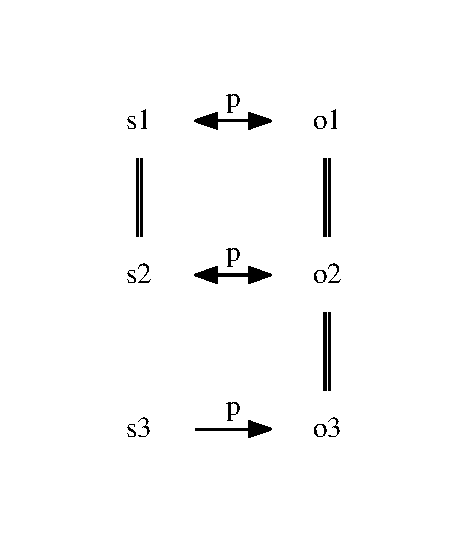
\includegraphics{./img/fixpoint_example}%[width=\columnwidth]
\caption{
  An illustrative example in which we show that defining
  $\underline{\approx}$ in terms of $\indp_{\approx}$ may not be optimal.
  The identity relation is represented with double-lined edges.
}
\end{figure}

%\begin{equation}
%\label{eq:10}
%\approx = \set{\pair{s_1}{s_2},\pair{o_1}{o_2},\pair{o_2}{o_3}}
%\end{equation}

The indiscernibility criteria for this example are shown
  in equation \ref{eq:20}.

\small
\begin{align}
\label{eq:20}
  \indp_{\approx}(\set{s_1,s_2,s_3})
=
  \indp_{\approx}(\set{o_1,o_2})
=
  \setdef{p^n}{\natnum{n}}
\end{align}
\normalsize

Based on the indiscernibility criteria in euqation \ref{eq:20} and
  the definition of the lower approximation
  (def. \ref{def:lower_approximation})
  we derive that the lower approximation for the example
  in figure \ref{fig:example} is empty.

If we change the relation that is used for calculating
  the closures of the predicate and object terms
  in the specification of the discernibility criteria,
  then the results for the lower approximation change.
According to the alternative definition \ref{def:lower_approximation2},
  there are two consistent solutions for the lower approximation:
  \begin{enumerate}
    \item $\lowerapprox_1 = \emptyset$,
          with $\indp_{\lowerapprox_1}(X) = \emptyset$
          for $X$ such that $\card{X} > 1$.
    \item $\lowerapprox_2 = \set{\pair{s_1}{s_2},\pair{o_1}{o_2}}$,
          with $\indp_{\lowerapprox_2}(\set{s_1,s_2,o_1,o_2}) = \setdef{p^n}{\natnum{n}}$
          and $\indp_{\lowerapprox_1}(X) = \emptyset$
          for all other $X$ such that $\card{X} > 1$.
  \end{enumerate}

Both solutions are correct,
  since both conform to the same strictures imposed by the framework.
It may also be reasonable to consider a greater lower approximation
  as more optimal, and the greatest lower approximation as most optimal.

\small
\begin{definition}
\begin{align}
\label{def:lower_approximation2}
  x_1 \lowerapprox x_2
\quad \iff \quad
  \forall_{\pair{y_1}{y_2} \in S_G^2}(\\
        \indp_{\lowerapprox}(\set{y_1,y_2})
      =
        \indp_{\lowerapprox}(\set{x_1,x_2})
    \rightarrow
      y_1 \approx y_2
  )\nonumber
\end{align}
\end{definition}
\normalsize

We have given an example for the lower approximation.
We expect that similar considerations apply to the higher approximation,
  where we maintain that the smallest higher approximation is
  the most optimal one.


